% ****** Start of file apssamp.tex ******
%
%   This file is part of the APS files in the REVTeX 4.1 distribution.
%   Version 4.1r of REVTeX, August 2010
%
%   Copyright (c) 2009, 2010 The American Physical Society.
%
%   See the REVTeX 4 README file for restrictions and more information.
%
% TeX'ing this file requires that you have AMS-LaTeX 2.0 installed
% as well as the rest of the prerequisites for REVTeX 4.1
%
% See the REVTeX 4 README file
% It also requires running BibTeX. The commands are as follows:
%
%  1)  latex apssamp.tex
%  2)  bibtex apssamp
%  3)  latex apssamp.tex
%  4)  latex apssamp.tex
%
\documentclass[%
 reprint,
%superscriptaddress,
%groupedaddress,
%unsortedaddress,
%runinaddress,
%frontmatterverbose, 
%preprint,
%showpacs,preprintnumbers,
%nofootinbib,
%nobibnotes,
%bibnotes,
 amsmath,amssymb,
 aps,
%pra,
%prb,
%rmp,
%prstab,
%prstper,
%floatfix,
spanish]{revtex4-1}

\usepackage{graphicx}% Include figure files
\usepackage{dcolumn}% Align table columns on decimal point
\usepackage{bm}% bold math
\usepackage{subcaption}
\usepackage[utf8]{inputenc}
\usepackage{tabularx}
%\usepackage{hyperref}% add hypertext capabilities
%\usepackage[mathlines]{lineno}% Enable numbering of text and display math
%\linenumbers\relax % Commence numbering lines

%\usepackage[showframe,%Uncomment any one of the following lines to test 
%%scale=0.7, marginratio={1:1, 2:3}, ignoreall,% default settings
%%text={7in,10in},centering,
%%margin=1.5in,
%%total={6.5in,8.75in}, top=1.2in, left=0.9in, includefoot,
%%height=10in,a5paper,hmargin={3cm,0.8in},
%]{geometry}
\graphicspath{ {imagenes/} }
\begin{document}

\preprint{APS/123-QED}

\title{Ising 2D por medio de sampléo Metrópolis-Montecarlo}% Force line breaks with \\
%\thanks{A footnote to the article title}%

\author{A.~Rabinovich}
 %\altaffiliation[Also at ]{}%Lines break automatically or can be forced with \\
\affiliation{%
 Departamento de F\'\i sica, Facultad de Ciencias Exactas y Naturales, Universidad de Buenos Aires,\\
 Pabell\'on I, Ciudad Universitaria, 1428 Buenos Aires, Argentina.
}%

%\collaboration{MUSO Collaboration}%\noaffiliation

\date{\today}% It is always \today, today,
             %  but any date may be explicitly specified

\begin{abstract}
Se estudió el comportamiento de una red 2D de spines utilizando el modelo de Ising y por medio de simulaciones Metrópolis-Montecarlo. Se obtuvo la magnetización, la energía media, el calor específico 
y la susceptibilidad magnética para redes de $L=32$, $L=64$, $L=128$, $L=256$ para un hamiltoniano con interacciones ferromagnéticas a primeros vecinos. Se halló una transición de fase para 
una temperatura crítica $T_c\approx2,36$ en buena concordancia con el valor teórico de $T_c\approx2,27$.
Se estudió además el fenómeno de frustración magnética utilizando un hamiltoniano con interacciones antiferromagneticas a segundos vecinos.
\end{abstract}

\maketitle

%\tableofcontents


\section{Introducción}
En ciertos metales como el hierro y el níquel, se observa la aparición de un momento magnético de caracter macroscópico, producido por la polarización espontánea en la misma dirección y sentido de 
una fracción 
de los spines de los átomos que constituyen el material. Esta magnetizacion espontánea se conoce como ferromagnetismo y es un efecto que solo se observa para temperaturas por 
debajo de 
una temperatura crítica $T_c$, llamada Temperatura de Curie. Para temperaturas mayores a $T_c$, la agitación térmica de las partículas
no permite un ordenamiento espontáneo de los spines. Se observa además que a medida que la temperatura se acerca a $T_c$, el calor específico del material se incrementa arbitrariamente, lo que 
sugiere que en la Temperatura de Curie ocurre una transición de fase de un estado ordenado a uno desordenado.\cite{huang}

\section{El modelo}
La descripción teórica más sencilla del ferromagnetismo es el modelo de Ising, modelo propuesto por Wilhelm Lenz en 1920 para el estudio de la magnetización de materiales ferromagnéticos 
como el hierro. En Ising 2D, se modela al material como un arreglo cuadrado de spines fijos donde cada spin puede tomar dos valores distintos: $s_i= \pm$1, figura \ref{fig:red_spines}, teniendo en 
cuenta la interacción de cada spin con sus vecinos. El hamiltoniano del modelo es por lo tanto:

\begin{equation}
H=-\sum_{<ij>}{Js_is_j}-\sum_{<ij>}{J's_is_j}-B\sum_{i}{s_i},
\label{hamiltoniano}
\end{equation}

donde $J$, la constante de acoplamiento modela la interacción entre un spin y sus primeros vecinos, $J'$ modela la interacción entre un spin y sus segundos vecinos y $B$ es un campo magnético 
externo. 

\begin{minipage}{0.45\textwidth}									
\centering
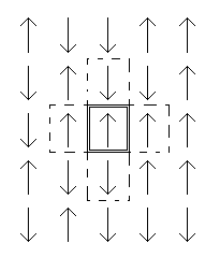
\includegraphics[width=0.4\textwidth]{imagenes/red_spines}
\captionof{figure}{Arreglo de spines fijos en el modelo de Ising. La línea punteada indica los primeros vecinos del spin encerrado por doble línea. Tomado de Muglia\cite{muglia}.}
\label{fig:red_spines}
\end{minipage}

En este trabajo utilizaremos $J$ y $J'$ isótropos. Para $J>0$ el material es ferromagnético mientras que para $J<$ 0 el material es antiferromagnético. Éste hamiltoniano favorece que 
los spines estén alineados, porque si $s_i=s_j$ entonces la energía disminuye en una cantidad $J$.\\
En el modelo de Ising 2D la temperatura crítica $T_c$ para $B=0$ y $J'=0$ puede ser obtenida de forma analítica mediante la ecuación \cite{onsager}:

\begin{equation}
T_c = \frac{J}{k_B}\frac{2}{ln(2+\sqrt{2})},
\label{T_c}
\end{equation}
con $k_B$ la constante de Boltzmann. Tomando $\frac{J}{k_B}=1$ se obtiene $T_c\approx2.27$ adimensional. A lo largo de éste trabajo se utilizará $J^*=\frac{J}{k_BT}$, una $J$ reducida adimensional.

\section{Programa de simulación del modelo de Ising}
El valor de expectación de un observable $A$ está dado por:
\begin{equation}
\langle A \rangle=\sum_{\nu}{A_{\nu}p_{\nu}},
\label{A}
\end{equation}
donde $A_{\nu}$ es el valor de $A$ en el estado $\nu$ y $p_{\nu}$ es la probabilidad de que el sistema se encuentre en ese estado, por lo tanto, dado un sistema con una cantidad discreta de estados, se podría calcular $A_{\nu}$ para todos los estados y calcular su promedio pesado.\\
La probabilidad de que un sistema de spines se encuentre en alguna configuración $\{s_\nu\}$ con energía $E\{s_\nu\}$ se puede obtener a partir del ensamble canónico y está dada por:
\begin{equation}
p_{\nu}=\frac{e^{-\beta E\{s_{\nu}\}}}{\sum_{\nu}e^{-\beta E\{s_{\nu}\}}}
\label{p_nu}
\end{equation}
con $\beta=\frac{1}{k_BT}$.\\
Sin embargo, para un sistema simple como el de Ising 2D, con  por ejemplo $L=20$, se tienen $2^{400}$ estados diferentes del sistema, por lo que resulta imposible examinarlos todos.\\
Para resolver éste inconveniente se puede realizar un muestréo o sampléo de algunos de los posibles estados del sistema. Para poder decidir qué estados samplear, utilizaremos el algoritmo de Metrópolis-MonteCarlo. En el mismo, en lugar de elegir estados al azar $\nu$, calcular $A_{\nu}$ y pesarlo por su probabilidad, se eligen los estados con probabilidad $p_{\nu}$ y se pesan todos con la misma probabilidad\\
Se escribió un código de simulación del modelo de Ising, empleando el algoritmo Metrópolis MonteCarlo en una red bidimensional cuadrada de espines, para obtener una colección representativa de distintos estados del ensamble canónico. Se impusieron condiciones de contorno periódicas para estudiar la magnetización en el seno de un material magnético.
El algoritmo Metrópolis se puede desglosar en:

\begin{enumerate}
\item{Se elige una configuración inicial de la red asignando 1 o -1 a cada spin de la misma de forma uniformenente aleatoria.}
\item{Se elige una temperatura $T$.}
\item{Se elige un spin de la red y se lo invierte (la elección puede ser aleatoria o secuencial).}
\item{Se calcula la energía de la nueva configuración y se la compara con la energía de la configuración en el paso anterior.}
\item{Si la energía disminuye, se acepta la nueva configuración del sistema.}
\item{Si la misma no disminuye, se acepta el nuevo estado con probabilidad $e^{-\beta \Delta E}$}
\item{Se itera desde el punto (3) K veces.}
\end{enumerate}

En particular nos interesa calcular la energía por spin $u$ y la magnetización por spin $m$ estudiando su variación en función de la temperatura $T$.
La energía se puede calcular como:

\begin{equation}
u=\frac{\sum_{\nu}{E_{\nu}\ p_{\nu}}}{N}
\label{energia}
\end{equation}

Mientras que $m$ es:

\begin{equation}
m=\frac{\sum_{\nu}{M_{\nu}\ p_{\nu}}}{N}
\label{magnetizacion}
\end{equation}
donde $M_{\nu}=\frac{\#s_{\nu}\uparrow-\#s_{\nu}\downarrow}{\#s}$

Como cada valor de spín puede tomar únicamente dos valores, hay un total de $2^N$ estados para una red
de $N$ espines, con lo cual calcular en forma exacta las ecuaciones (\ref{energia}) y (\ref{magnetizacion}) puede volverse computacionalmente
costoso. Por ello, tomaremos en cuenta sólo los estados que contribuyan mayoritariamente, tal cual se discutió anteriormente.\\
Teniendo eso en cuenta, la energía $u$ se puede calcular con la siguiente aproximación:

\begin{equation}
u=\frac{1}{NK}\sum_{i=1}^{K}{E_i},
\label{emedia}
\end{equation}

donde $E_i$ es la energía obtenida en el i-ésimo paso.
Análogamente para $m$:

\begin{equation}
m=\frac{1}{NK}\sum_{i=1}^{K}{M_i},
\label{mmedia}
\end{equation}

Además puede demostrarse que la susceptibilidad magnética, definida como $\chi =\frac{\partial{M}}{\partial{B}}$ se puede calcular como:

\begin{equation}
\chi=\beta \left( \langle m^2 \rangle - \langle m \rangle ^2 \right)
\label{ec:susc}
\end{equation}

y en forma análoga, el calor específico a volumen
constante $c_v$ =$\frac{\partial{U}}{\partial{T}}$ se puede calcular como:

\begin{equation}
c_v = \beta ^2 \left(\langle u^2 \rangle -\langle u \rangle ^2 \right)
\label{ec:calor}
\end{equation}

\section{Resultados}
Las primeras muestras tomadas no son representativas del sistema físico ya que cada muestra difiere en solo
un espín. Se debe dejar al sistema llegar al equilibrio, tomando un número de pasos suficientemente grande (idealmente infinito). 

\subsection{Termalización}
Al comenzar el algoritmo, el sistema se encuentra en punto del espacio de fases que no tiene porque ser un estado típico del sistema en equilibrio a una cierta temperatura. Después de hacer cierto número de flipeos (invertir un spin de la red), el sistema llega a encontrarse 
en un punto del espacio de fases en el cual los valores de la energía del sistema rondan el valor más probable. A éste proceso se lo conoce como termalización. En la figura \ref{termalizacion} se muestra la termalización para una red de $L=256$, $J=J'=0$, $B=1$ y $T=5$. Se observa que a partir de aproximadamente 150000 pasos de montecarlo, la magnetización del sistema alcanza la magnetización teórica dada por $tanh(B)=tanh(1)\approx0.19$, por lo que se decidió termalizar todas las redes con 150000 flips.\\
Debido a que los pasos de la temperatura utilizados en cada experiencia fueron de $\Delta T = 0.1$, comenzando desde $T=5$, fue suficiente termalizar al comienzo una única vez.

\begin{minipage}{0.45\textwidth}									
\centering
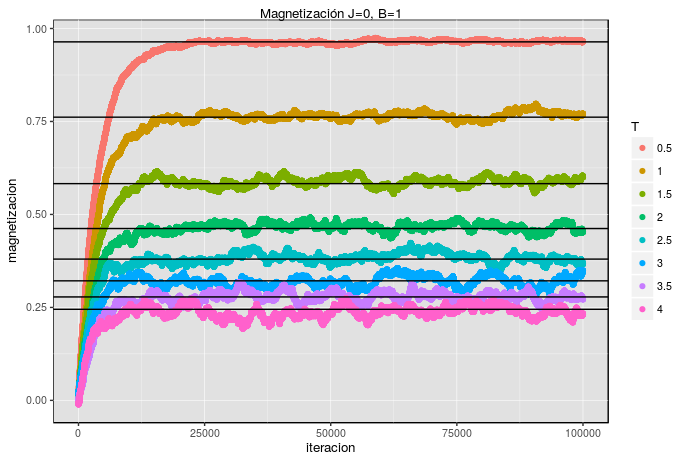
\includegraphics[totalheight=0.25\textheight]{imagenes/termalizacion/magnetizacion.png}
\captionof{figure}{Termalización en una red de L = 256}
\label{termalizacion}
\end{minipage}

\subsection{Autocorrelación}
Debido a que cada muestra difiere únicamente en un spin de la anterior, las muestras están altamente correlacionadas y pueden no resultar representativas. Para poder tomar entonces muestras representativas, se calculó el coeficiente de autocorrelación dado por:

\begin{equation}
\rho = \frac{\langle(x_i-\mu)(x_{i+k}-\mu)\rangle}{\langle(x_i-\mu)^2\rangle}
\label{ec:autocorrelacion}
\end{equation}

con $x_i$ la magnetización o la energía en el paso i-esimo y $x_{i+k}$ en el paso i+k-esimo.\\
Se calculó la autocorrelación tomando $k=0,...,30000$ para una red de $L=128$, $J=1$, $J'=0$, $B=0$ y para $T=5$, $T=3$ y $T=1.5$ y se graficó $\rho$ vs. $k$, figura \ref{fig:autocorrelacion}.

\begin{minipage}{0.45\textwidth}									
\centering
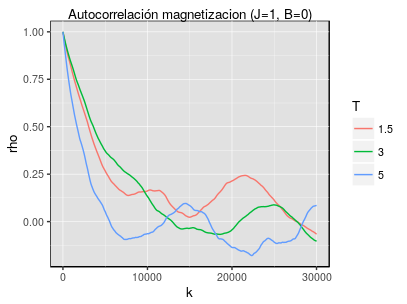
\includegraphics[totalheight=0.25\textheight]{imagenes/autocorrelacion/energia.png}
\captionof{figure}{Autocorrelación para una red de L=128}
\label{fig:autocorrelacion}
\end{minipage}

Se observa que a partir de $k=15000$ la autocorrelación es cercana a cero para todas las temperaturas. Por lo tanto, se tomó una muestra cada 15000 iteraciones de metrópolis como muestra representativa.

\subsection{Magnetización espontánea y susceptibilidad}
Para una red de $L=128$, comenzando desde $T=5$ hasta $T=0.5$ y disminuyendo la temperatura con $\Delta T=0.1$, se realizaron 10000000 de iteraciones de MonteCarlo para cada temperatura, termalizando únicamente para $T=5$. Se tomaron aproximadamente 650 muestras por temperatura y con ellas se calculó la magnetización media por temperatura. Se graficó un histograma de las magnetizaciones obtenidas, cómo se visualiza en la figura \ref{fig:magnetizacion_sin_corona}.   

\begin{minipage}{0.45\textwidth}									
\centering
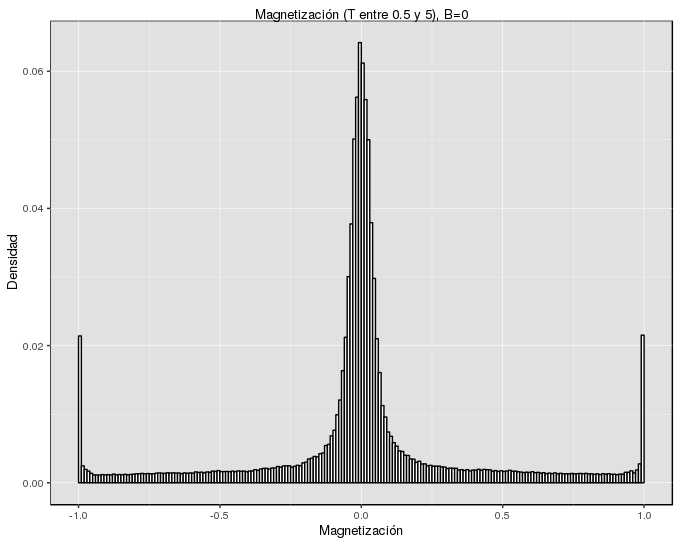
\includegraphics[totalheight=0.25\textheight]{imagenes/sin_corona/magnetizacion.png}
\captionof{figure}{Magnetización media por partícula en función de la temperatura para una red de L=128}
\label{fig:magnetizacion_sin_corona}
\end{minipage}

Se observa una distribución bimodal de la magnetización, lo que implica la existencia de una simetría en la magnetización espontanea, dado que resulta indistinto para el sistema que los spines se polaricen hacia arriba o hacia abajo.\\
Para poder romper ésta simetría, se agregó una corona alrededor de la red con spines fijos apuntando hacia arriba. Para redes de tamaño infinito, la corona tiene medida nula y por lo tanto no modifica 
los valores medios calculados. Sin embargo, alcanza para romper la simetría del sistema y lograr que la magnetización quede distribuida alrededor de uno solo de los mínimos.
Se realizó el mismo cálculo anterior para redes de $L=32$, $L=64$, $L=128$ y $L=256$, obteniéndose los valores observados en la figura \ref{fig:magnetizacion_con_corona}

\begin{minipage}{0.45\textwidth}									
\centering
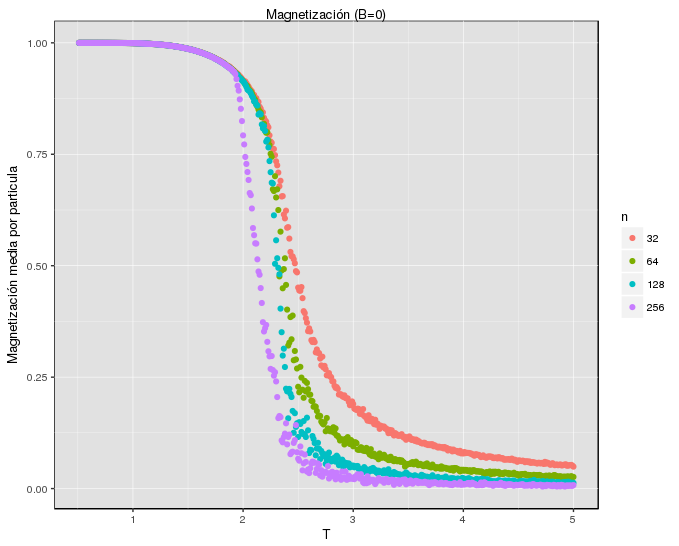
\includegraphics[totalheight=0.25\textheight]{imagenes/con_corona/magnetizacion.png}
\captionof{figure}{Magnetización media por partícula en función de la temperatura para redes de distinto lado L}
\label{fig:magnetizacion_con_corona}
\end{minipage}

La magnetización neta es máxima y constante para temperaturas bajas ($T<T_c$), correspondiente a un estado del sistema con todos
los espines alineados al producirse la magnetización espontánea, y luego se ve una súbita disminución de la magnetización
para temperaturas alrededor de la temperatura crítica $T_c$, para luego ser prácticamente nula para temperaturas mayores. Esto se corresponde con una alineación aleatoria de los spines producto de la agitación térmica del sistema.
Análogamente al caso anterior, el cambio repentino de la magnetización se relaciona con una variación brusca en la susceptibilidad magnética. En la
figura \ref{grafico_susceptibilidad_magnetica} se graficó la susceptibilidad en función de la temperatura, donde se observa un pico en los valores de temperatura en donde ocurre el cambio en la magnetización, en los valores esperados para la $T_c$.

\begin{minipage}{0.45\textwidth}									
\centering
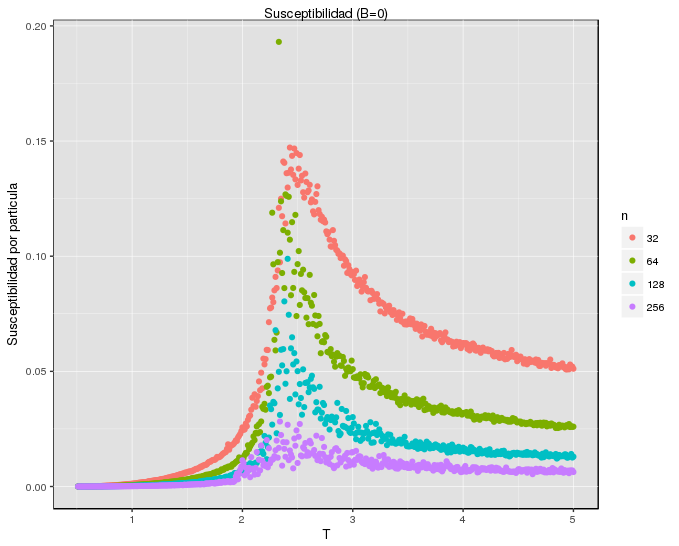
\includegraphics[totalheight=0.25\textheight]{imagenes/con_corona/susceptibilidad.png}
\captionof{figure}{Susceptibilidad magnética por partícula en función de la temperatura para redes de distinto lado L}
\label{grafico_susceptibilidad_magnetica}
\end{minipage}

\subsection{Energía media y calor específico}

En la figura \ref{ref:grafico_energia} se graficó la energía media en función de la temperatura para redes de $L=32$, $L=64$, $L=128$ y $L=256$. Se observa nuevamente que a temperaturas bajas, el sistema presenta una energía mínima y constante. Esto sucede cuando los espines se alinean al presentarse una magnetización espontánea.

\begin{minipage}{0.45\textwidth}									
\centering
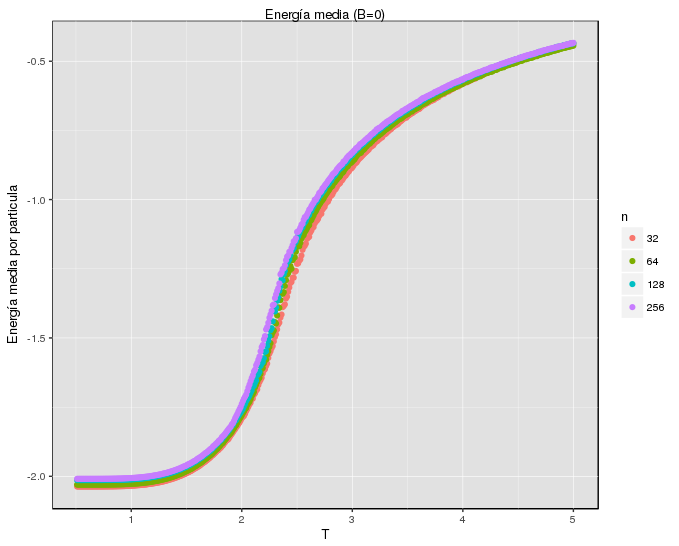
\includegraphics[totalheight=0.25\textheight]{imagenes/con_corona/energia.png}
\captionof{figure}{Energía media por partícula en función de la temperatura para redes de distinto lado L}
\label{ref:grafico_energia}
\end{minipage}

Se observa que la energía comienza a aumentar para $T=1.5$ y alrededor de la $T_c$ se observa un brusco cambio de la energía del sistema junto con un cambio de concavidad en la curva de energía. Aumentando la temperatura respecto de la $T_c$, se obtiene un aumento monótono de
la energía. Asociado a este cambio brusco en la energía alrededor de la $T_c$, debe existir un pico en el calor
específico del sistema. En la figura \ref{grafico_capacidad_calorifica} se graficó el calor específico en función de la temperatura. Se observa un máximo alrededor de la temperatura $T_c$ para todas las redes.

\begin{minipage}{0.45\textwidth}									
\centering
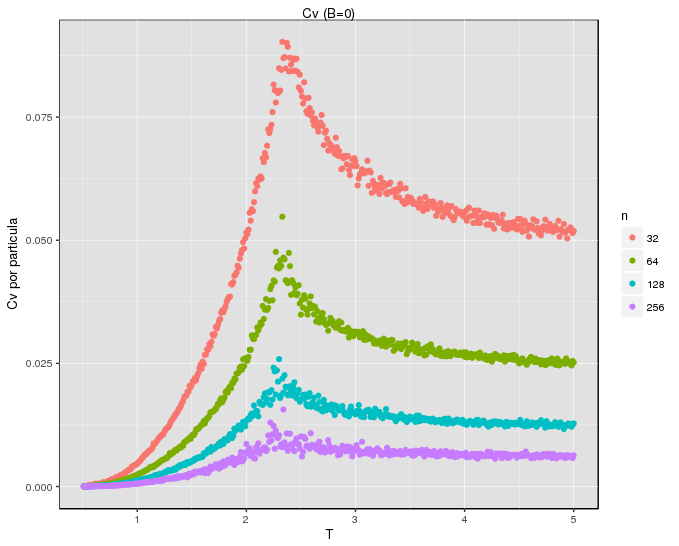
\includegraphics[totalheight=0.25\textheight]{imagenes/con_corona/cv.png}
\captionof{figure}{Capacidad calorífica por partícula en función de la temperatura para redes de distinto lado L}
\label{grafico_capacidad_calorifica}
\end{minipage}

Para encontrar la temperatura $T_c$, se ajustó por medio de un polinomio de grado 20 el calor específico para la red de L = 64. Luego se buscó el pico obteniéndose un máximo en $T_c\approx2.36$, en 
buena concordancia con el calculado en \ref{T_c}. 
En la figura \ref{capacidad_calorifica_con_ajuste_polinomial} se observa un gráfico del calor específico para la red de L = 64 y el polinomio de ajuste.

\begin{minipage}{0.45\textwidth}									
\centering
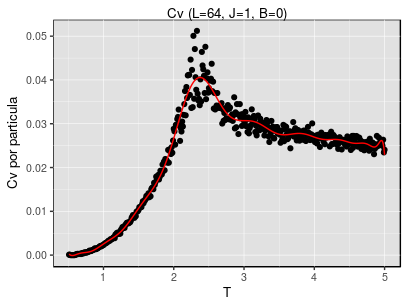
\includegraphics[totalheight=0.25\textheight]{imagenes/con_corona/ajuste_cv.png}
\captionof{figure}{Capacidad calorífica por partícula en función de la temperatura para una red de L = 64 y ajuste polinomial}
\label{capacidad_calorifica_con_ajuste_polinomial}
\end{minipage}

\subsection{Hamiltoniano con segundos vecinos y fenómeno de frustración}
El fenómeno de frustración es una característica de los sistemas magnéticos que lleva a estructuras complejas. Éste fenómeno se produce por un conflicto en la interacción entre spines en la red, en 
donde la alineación de un spin con sus primeros vecinos reduce la energía de interacción entre ellos, pero la aumenta con sus segundos vecinos. Por ejemplo, en la red 2D, tomando un spin y suponiendo 
que todos sus primeros vecinos apuntan hacia arriba y sus segundos vecinos apuntan hacia abajo, con acoplamientos ferromagneticos para sus primeros vecinos y anti para sus segundos, el spin es 
frustrado porque cualquiera de sus dos orientaciones dan la misma energía. El spin no puede minimizar en simultaneo la energía con todos sus vecinos.\\
Tomando en el hamiltoniano de \ref{hamiltoniano} $J=1$, $B=0$ y $J'=-1$ se obtiene un hamiltoniano con interacciones ferromagnéticas a primeros vecinos y antiferromagneticas a segundos vecinos, 
para estudiar el fenómeno de frustración en el modelo de Ising.\\ 
En la figura \ref{fig:frustracion} se graficó la magnetización media en función de la temperatura para una red de $L=64$. Se observa que no existe magnetización espontanea en el rango de temperaturas 
estudiado.

\begin{minipage}{0.45\textwidth}									
\centering
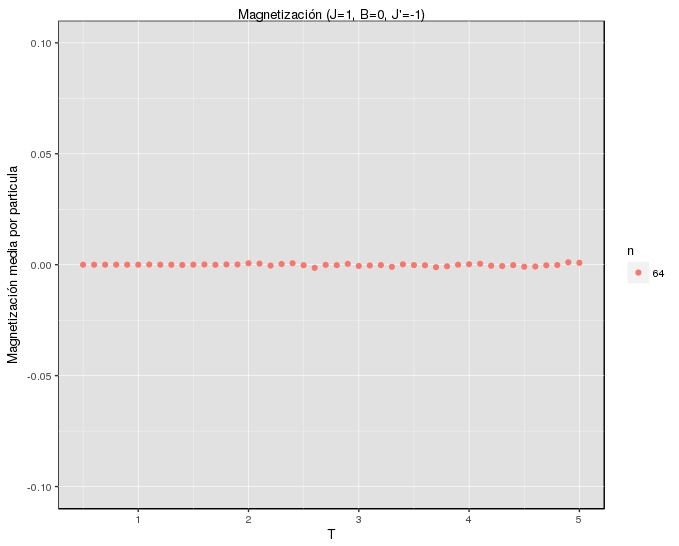
\includegraphics[totalheight=0.25\textheight]{imagenes/frustracion/magnetizacion}
\captionof{figure}{Magnetización por partícula en función de la temperatura para una red de L = 64 a segundos vecinos.}
\label{fig:frustracion}
\end{minipage}

Ésto es consistente con la frustración magnética, producto de la incapacidad de minimizar la energía a primeros y segundos vecinos en simultaneo para las interacciones elegidas. 

\section{Conclusiones}
Se estudió el comportamiento de una red 2D de spines utilizando el modelo de Ising y por medio de simulaciones Metrópolis-Montecarlo. Se obtuvo la magnetización, la energía media, el calor específico 
y la susceptibilidad magnética para redes de $L=32$, $L=64$, $L=128$, $L=256$ para un hamiltoniano con interacciones ferromagnéticas a primeros vecinos. Se encontró un salto en la magnetización 
espontanea y una divergencia en el calor específico para una temperatura crítica $T_c$, señal de una transición de fase. Se halló que la transición de fase ocurre para temperaturas de 
$T_c\approx2,36$ al ajustar por un polinomio el máximo del calor específico para una red de 64x64 spines, en concordancia con el valor teórico de $T_c\approx2,27$. La diferencia en las temperaturas 
obtenidas puede ser atribuida a efectos de tamaño finito en las redes utilizadas.\\
Se estudió además el fenómeno de frustración magnética utilizando un hamiltoniano con interacciones antiferromagneticas a segundos vecinos, obteniendose efectivamente una anulación de la 
magnetización espontanea en el rango de temperaturas estudiado.

\begin{acknowledgments}
A. Rabinovich es becario doctoral del CONICET. 
\end{acknowledgments}

\appendix
\bibliography{ising}% Produces the bibliography via BibTeX.

\end{document}


